\chapter{等式松弛机制}\label{chap:method2}

本章节主要介绍局部搜索算法在LS\_NRA处理等式约束时的松弛技术,主要可以分为两个阶段:松弛阶段和恢复阶段。
首先,本章节考虑到局部搜索迭代算法的效率问题,引入赋值复杂度的概念,并提出非线性实数理论独有的无理数赋值挑战。
紧接着,本文提出一种等式松弛方法来暂时扩大约束的可行域,从而保证了有理数赋值,使得算法可以找到附近的近似解。
然后,本文探讨了算法最后的恢复阶段,即近似解如何恢复为原问题的精确解,并提出了具体的懒惰版本的实现方法。
最后,本文介绍了其他的一些可行的改进策略。

\section{代数数赋值的复杂度}
在SMT问题的四种主流算术理论(线性整数理论、线性实数理论、非线性整数理论、非线性实数理论)中,非线性实数理论(NRA)因为其存在高次多项式约束与潜在的无理数赋值问题而最难处理。这些情况基本发生在等式约束上,例如$x^2 + y^2 = 2$等。对于局部搜索迭代而言,尽管在计算机中可以使用代数数表示无理数,但无理数赋值问题带来的仍是多项式评估的效率低下,进而影响到实根隔离与计算可行域等操作。除此之外,一些分母较大的代数数仍然会影响计算速度。

以往的工作\cite{multilinear,LiXZ23}都尽量避免了代数数引发的计算问题,因此将非线性问题限定为多线性约束(multilinear)或至少包含一个线性项的等式约束上。其中,工作\cite{multilinear}考虑了有理数赋值的分母大小问题,并将其作为操作得分相同时的打破平均策略。

我们的工作考虑了非线性实数的全部测试样例,一个关键的优化是尽量减少复杂赋值的出现频率。为此,我们首先定义赋值之间的复杂度关系如下:

\begin{definition}{\textbf{赋值复杂度(Complexity of values)}}
\label{def:complexity}
我们定义代数数上的偏序$\prec_c$如下。$x \prec_c y$当且仅当以下任何一种情况成立:

\begin{itemize}
    \item $x$和$y$都是有理数,且$x$的分母小于$y$的分母。
    \item $x$是有理数,而$y$是无理数。
\end{itemize}
当$x \prec_c y$或者$y \prec_c x$均不成立时,我们认为$x$和$y$的复杂度相当,记为$x \sim_c y$。
\end{definition}

\section{松弛机制}
我们将等式的松弛机制简单描述如下:每次当等式或者不等式约束迫使某一个变量必须赋值为一个相对复杂的代数数时,我们会暂时松弛这些约束,使用复杂度相对低的松弛解,然后以松弛的形式继续局部搜索的迭代过程。在具体实现上,我们引入以下两个参数来设置算法门槛:
\begin{itemize}
    \item $\epsilon_v$:根据定义\ref{def:complexity}衡量表示代数数复杂度,取值为$10^{-4}$。
    \item $\epsilon_p$:多项式约束松弛的程度,见定义\ref{def:relaxation},取值为$10^{-4}$。
\end{itemize}


需要注意的是,在非线性实数理论中,无理数赋值并不完全由等式约束所要求,可能是多个形如$p \ge 0$或$p \le 0$的约束交集所决定。因此,本文实际上讨论的是严格多项式的松弛问题。具体的松弛机制定义如下:

\begin{definition}{\textbf{约束松弛(Relaxation of constraints)}}
\label{def:relaxation}
\begin{itemize}
    \item 如果约束形如$p = 0$,将其松弛为$p < \epsilon_p$和$p > -\epsilon_p$。
    \item 如果约束形如$p \ge 0$,将其松弛为$p > -\epsilon_p$。同样的,如果约束形如$p \le 0$,将其松弛为$p < \epsilon_p$。
\end{itemize}
\end{definition}

在局部搜索迭代中,当我们计算某个变量$v$的分数时,如果最优的分数来自于一个点区间,我们会记录这个点区间对应的边界子句标号。如果变量$v$在后续的迭代中被选中,并且其赋值比之前的赋值和$\epsilon_v$的复杂度高,那么记录的等式约束和严格不等式约束都会被松弛。也就是说,我们的松弛机制是懒惰的,只有当无理数赋值十分必要时才会进行,而非直接在预处理阶段进行。当松弛之后,局部搜索算法继续迭代,并且文字和多项式的评估完全按照松弛后的形式进行。


\section{恢复机制}
当局部搜索算法找到了一个松弛形式下的“可行解”之后,这个解被称为\textbf{近似解}。事实上,这并不能确保精确解的存在,鉴于SMT问题的要求,我们仍然需要找到原始状态下的附近精确解。图\ref{fig:relaxation}给出了等式松弛和恢复的示意图。本工作主要尝试两种方法。

\subsection{第一种恢复方法:基于等式约束结构的链式恢复}
第一种方法是对于松弛状态下的约束进行启发式分析,尝试找到一种可以满足所有等式的变量信息。整体的分析步骤如下:
\begin{enumerate}
    \item 如果任意一个变量目前赋值为0,将其代入到所有的约束中,用来化简多项式的复杂项。
    \item 删除所有形如$p \cdot x + q = 0$等式约束中的变量$x$,其中$p$在当前赋值下的评估不接近0。
    \item 最后,我们迭代地寻找只出现在一个等式约束的变量。我们将变量与对应的等式约束相关联,然后在迭代中忽略该等式(因为该等式的可满足性可以由这个变量直接决定)。
\end{enumerate}
当步骤3中不存在等式约束时,我们尝试在上述步骤中以倒序顺序求解变量。我们首先考虑步骤3中的变量-等式关联,利用这种等式约束直接求解这些变量的赋值。然后我们在步骤2中求解其余变量的赋值。最后我们检查所有子句的可满足性。我们形式化地将变量和等式之间的关系定义为如下有向图:
\begin{definition}{\textbf{等式约束关系图 (Equality Relation Graph)}}
考虑逻辑公式$\Phi$,我们定义等式关系图$G$如下:
\begin{itemize}
    \item \textbf{顶点:}所有出现在等式关系中的变量均视为一个顶点。
    \item \textbf{有向边:} 对于$\Phi$中每一个形如$x_{eq}: p \cdot x + q = 0$的等式约束,记$V(x_{eq})$为约束包含的所有变量,我们将变量$x$与等式约束$x_{eq}$相关联。我们为变量$V(x_{eq}) \setminus \{x\}$到$x$的每一对变量创建有向边,即$\forall x_{eq}: \forall v \in V(x_{eq}) \setminus \{x\}, v \xrightarrow{x_{eq}} x$。其意义是每一个有向边起点的赋值将有助于终点变量赋值的推理。
\end{itemize}
\end{definition}

第一种方法可以理解为优先对入度为0的变量进行赋值推理,然后根据有向边的关系进行图上的传播。例\ref{ex:restore1}给出了一个直观的例子。

\begin{figure*}[t]
    \centering
    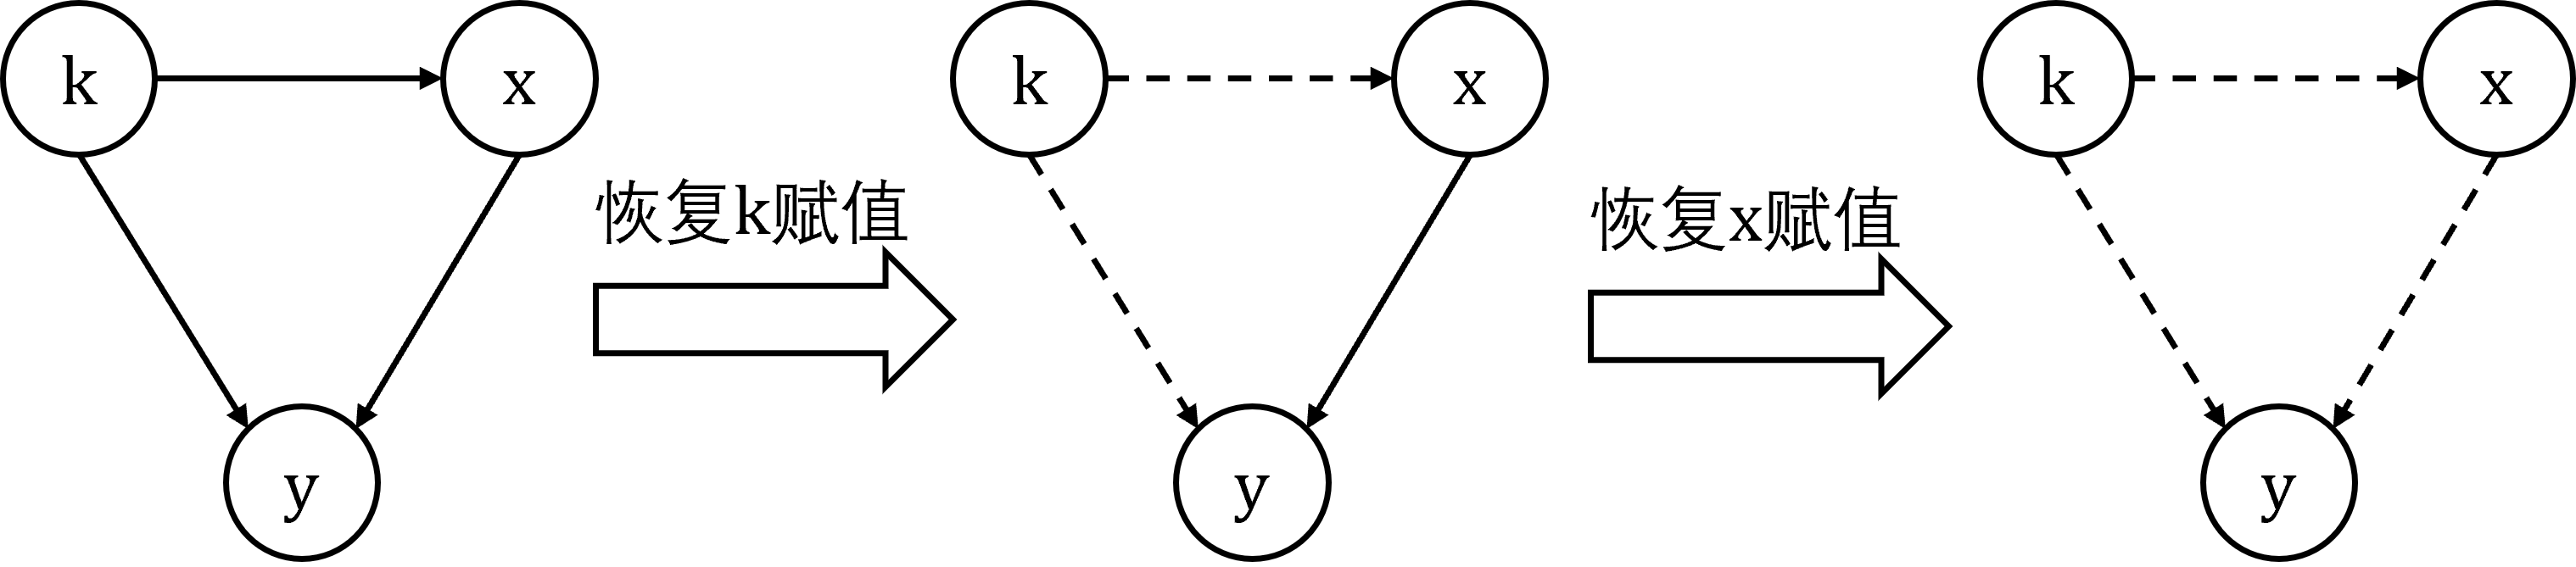
\includegraphics[width=\columnwidth]{Img/restore1.png}
    \bicaption {等式约束关系图。} {Demo of equality constraint graph.}
\label{fig:restore1}
\end{figure*}


\begin{example}
\label{ex:restore1}
假设当前近似解为$\{k \mapsto 1, x \mapsto 1, y \mapsto 1\}$,且有如下等式约束:$\{P_1: (k^2 + 3k) x + 6k = 0, P_2: k^2 x^2 + 3y = 0\}$。约束$P_1$和$P_2$可以分别关联变量$x$和$y$,我们建立等式关系图如图\ref{fig:restore1}。
\begin{enumerate}
    \item 建立变量和等式约束关联:$x \sim P_1, y \sim P_2$
    \item 考虑当前节点的入度,变量$k$的入度为0,不被等式所限制,变量$x$的入度为1,受变量$k$的赋值直接影响,变量$y$的入度为2,受变量$x$和$k$的赋值直接影响。
    \item 从自由变量$k$开始考虑,消去起点为$k$的有向边,此时变量$x$的入度为0。
    \item 推断$x \mapsto -1.5$,赋值后消去起点为$x$的有向边。
    \item 此时变量$y$的入度为0,推断赋值为$y \mapsto -0.75$。
    \item 检查当前赋值$\{k \mapsto 1, x \mapsto -1.5, y \mapsto -0.75\}$满足所有约束。
\end{enumerate}
\end{example}


\subsection{第二种恢复方法:小范围局部搜索}
当第一种方法不能解决所有等式约束可满足状态时,我们使用第二种方法进行恢复。第二种方法使用一种简化版本的局部搜索算法(limited local search)来尝试将近似解移动到最终的精确解。首先,我们把所有松弛的约束恢复为起始状态,然后继续在算术变量上运行局部搜索,直到找到了一组精确解或者局部搜索没有改进为止。相比于主流程中的局部搜索,恢复阶段的局部搜索算法是一种局限的版本,因为我们舍弃了布尔变量的迭代,以及一些随机步骤的发生。并且在实际运行中,近似解往往已经满足了绝大多数约束,因此受限版本的局部搜索算法只聚焦于几个尚且没有满足的等式约束,迭代的速度和运行效率要快很多。相比于第一种方法,第二种方法一般用于等式约束传播不为明显的情况,例\ref{ex:restore2}给出了一种情况。

\begin{example}
考虑逻辑公式$\Phi = x^2 + y^3 = 8 \wedge 2x^2 - 3y^2 > 6$,目前的近似解为$\{x \mapsto 12, y \mapsto -1.54\}$,仅满足松弛等式约束和不等式约束。恢复为原始状态后,等式约束不再满足,开始进行局部搜索。
\begin{itemize}
    \item 考虑针对原始等式约束固定变量$x$和$y$的两种关键移动,因为赋值复杂度的考量,选择操作$\{y \mapsto -\sqrt[3]{136}\}$
    \item 经过检查,赋值同时满足两个约束,找到精确解$\{x \mapsto 12, y \mapsto -\sqrt[3]{136}\}$。
\end{itemize}
\label{ex:restore2}
\end{example}

算法\ref{alg:relaxation}展示了加入了松弛机制后的局部搜索算法。和以往算法的主要区别在于,当一个变量的赋值复杂度超过了$\epsilon_v$时,等式约束会被松弛。当所有的约束都被满足时(找到了近似解),根据松弛约束的结构(第一种恢复方法)尝试找到附近的一个精确解。如果此方法失败,我们尝试局限版本的局部搜索(第二种方法),直到找到一个精确解或者局部搜索没有改进为止。如果以上尝试均失败,尝试使用一种新的赋值方式重启。

\begin{figure*}[t]
    \centering
    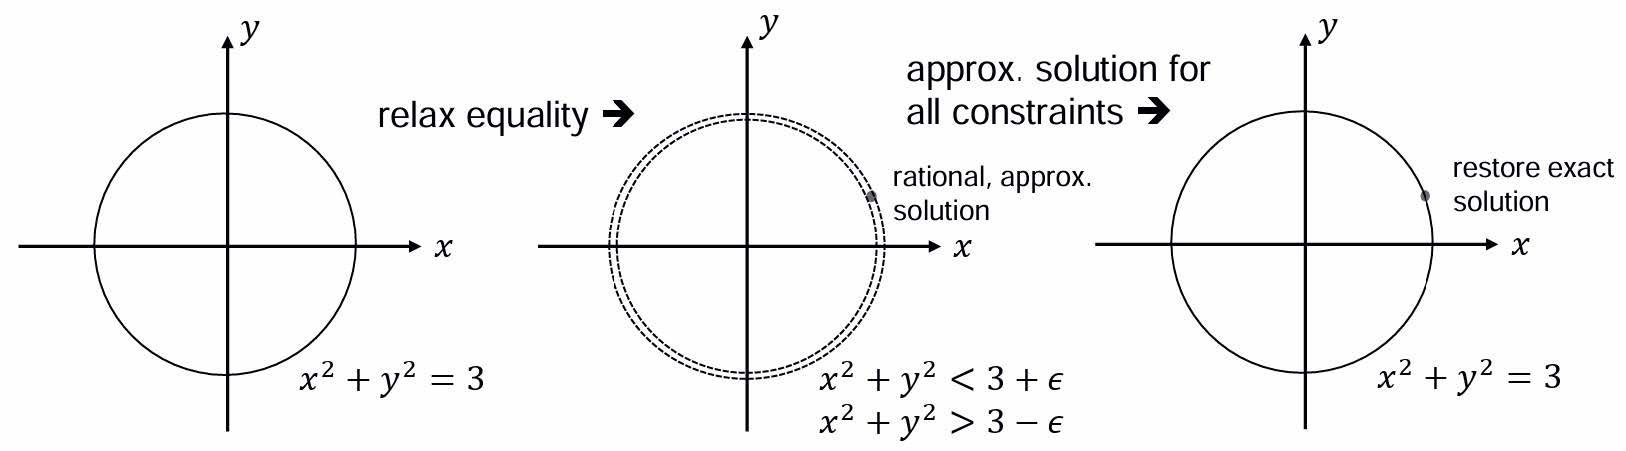
\includegraphics[width=\columnwidth]{Img/relax.jpg}
    \bicaption {等式松弛和恢复机制示意图。} {Demo of relaxation and restoration for equalitiy constraints.}
\label{fig:relaxation}
\end{figure*}

实际上,我们在实验中发现两种寻找精确解的启发式方法在不同场景下有不同的用处。第一种基于等式约束结构的方法在涉及到线性方程时表现很好。第二章方法能够很好地处理变量存在多个赋值区域的情况,但是仍然很难保证同时满足所有的不等式约束。事实上,应用很多先进的方法来精确求解等式约束十分有前景\cite{CimattiGLS22, LiXZ23b}。但是,本文提出的方法仍然可以简单地拓展到更复杂的约束中,并且独立地验证精确解的存在。

\section{本章小结}
本章节主要讨论了LS\_NRA应对非线性实数算术特有的等式约束无理数赋值的解决策略。首先,本文回顾了以往工作中针对赋值复杂度的讨论,并进一步将这个概念拓展到代数数赋值上。然后,本文给出了等式松弛的概念,其原理是暂时扩大可行域来支持有理数赋值。最后,本文讨论了两种用于产生精确解的恢复算法,并讨论了两种算法的适用场景。

\begin{algorithm}[t]
    \caption{Relaxation of Equalities}
    \label{alg:relaxation}
    \textbf{Input}: A set of clauses $F$ \\
    \textbf{Output}: An assignment of variables that satisfy $F$, or failure
    
    \begin{algorithmic}[1] %[1] enables line numbers
        \Statex \hrulefill
        \STATE Initialize assignment to variables;
        \While {\top}
            \IF{all clauses satisfied}
            \STATE success \leftarrow find exact solution by analyzing structures;
            \IF{success}
            \RETURN success with assignment;
            \ELSE
            \STATE Restore relaxed constraints to original form;
            \STATE success \leftarrow limited local search;
            \IF{success}
            \RETURN success with assignment;
            \ELSE
            \STATE Perform major restart;
            \ENDIF
            \ENDIF
            \ENDIF

            \IF{time or step limit reached}
            \RETURN failure;
            \ENDIF

            \IF{no improvement for certain steps}
            \STATE Perform minor restart;
            \ENDIF
            
            \STATE Proceed algorithm as Algorithm \ref{alg:basic};
        \EndWhile

        \STATE \textbf{return} failure
    \end{algorithmic}
\end{algorithm}